\question[6] $13.(6$分)如图所示装置可以用来研究小车的匀变速直线运动.带有定滑轮的长木板放置在桌面上,重物通过跨过定滑轮的细线拉着小车向左加速运动,定滑轮与小车间的细线与长木板平行,打点计时器打下的纸带记录下小车的运动信息$.(1)$下面说法正确的是$______.A.$长木板必须水平放置B.小车的质量必须远大于重物的质量纸带$\C.$需要平衡小车与长木板间的摩擦力D.应该先接通打点计时器的电源,然后再释放小车(2)实验时将打点计时器接到频率为$50Hz$的交流电源上,选取一条点迹清晰的纸带,在纸带上每隔四个点取一个计数点,测出相邻计数点间的距离如图所示,其中$x_1=5.09cm,x_2=7.10cm,x_3=9.10cm,x_4=11.10cm,x_5=13.09cm,x_s=15.10cm.$则打第4个计数点时小车的速度$v_4=_m/s,$小车的加速度$a=_m/s^2($结果均保留两位有效数字).
\begin{center}
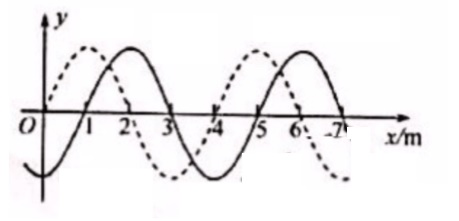
\includegraphics[]{img/image13.jpeg}
\end{center}

\question[6] $14.(9$分)某同学用如图所示装置做"探究加速度与合力关系"的实验.测得小车(带遮光片)的质量为M,当地的重力加速度为$g.\frac{2}{1}cm⊥$砂桶$1020(1)$实验前,用游标卡尺测出遮光片的宽度,示数如图所示,则遮光片的宽度为$d=__cm.(2)$为了使细线的拉力近似等于砂和砂桶的总重力,必须$_—°A.$将长木板的右端适当垫高,以平衡摩擦力B.砂和砂桶的总质量远小于小车的质量C.使连接小车的细线与长木板平行D.减小遮光片的宽度$(3)$调节好装置,将小车由静止释放,与光电门连接的计时器显示小车通过光电门时遮光片的遮光时间t,要测量小车运动的加速度,还需要测量$__($填写需要测量的物理量名称),若该物理量用x表示,则小车运动的加速度大小为$__($用测得的物理量符号表示$).(4)$保持小车每次释放的位置不变,光电门的位置不变,改变砂和砂桶的总质量,重复实验,测得多组小百投翻联显$2020$届$TOP300$七月尖子生联考物理第3页"共6页车通过光电门的遮光时间t及砂和砂桶的总质量m.为了使图象能直观地反映物理量之间的关系.应该作出$____$__($(-t^{\prime\prime},m-\frac{1}{t}m-t^{2},\cdotsm-\frac{1}{t^{2}}y$图象.当图象为过原点的一条倾斜的直线,表明质量一定时加速度与合力成正比.
\question[6] $15.(8$分)某物体沿着一条直线做匀减速运动.途经$A.B.C$三点,最终停止在D点$.A、B$之间的距离为$s…B.C$之间的距离为_号$\frac{2}{3}s_{0}$物体通过AB与BC两段距离所用时间都为t…求$:(1)$物体经过A点时的速度$,Aiⅳc―b(2)$物体经过CD段的平均速度.百以固获生$2020$届$TOP00$七月尖子生联考物理第4页共6页
\question[6] $16.(11$分)如图所示.质量为$m=6kg,$足够长的长木板放在水平面上,其上表面水平.质量为$m_1=3kg$的物块A放在长木板上距板右端$L,=3m$处,质量为$m=3kα$的物块B放在长木板上左端.地面上离长的$=,_=$原图的二一下下面平下列的^新出Ⅱ两气出A是得重是重的的=体图关色是不W的数用图新此正要用假的物对脱离个假已知四物块与长木板间的动摩擦因数均为$\mu_1=0.5,$长木板与地面间的动摩擦因数为$\mu_2=0.1,$重力加速度$g=10m/s^∘,$最大静摩擦力等于滑动摩擦力,不计物块大小,求拉力F的大小$._e_v─r.∥$
\question[6] $17.(13$分)质量为$1kg$的小型无人机下面悬挂着一个质量为$0.5kg$的小物块,正以$2m/s$的速度匀速下降,某时刻悬绳断裂小物块竖直下落,小物块经过2s落地,已知无人机运动中受到的空气阻力大小始终为其自身重力的$0.1$倍,无人机的升力始终恒定,不计小物块受到的空气阻力,重力加速度为$10m/s,$求出小物地刚要落地时$."'0¥10$的.O生人能到地面的高度$.(2)$无人机离3百以固获生$2020$届$TOP00$七月尖子生联考物理第5页共6页
\question[6] $18.15$分)如图所示,倾角为$37^°$的斜面体固定在水平面上,斜面上$A、B$两个位置之间的距离为$2m.$第一次用沿斜面向上,大小为$F=6N$的力把质量为$0.5kg$的物体由静止从A处拉到B处.所用时间为$1s,$第$"m"g×_"_0ⅲ$在段时间二场上$A+,$物是实验到B从$___"$时上_重石眼至不分物体运动到B处时速度刚好减为零.已知$sin37=0.6,cos37=0.8,$不计物体大小,重力m区段器二0"常有的因数$,(1)$物体与斜面间的动摩擦因数$.(2)$物体第二次从A运动到B的过程·水平力F的作用时间.(结果可保留根式)百以固获生$2020$届$TOP00$七月尖子生联考物理第5页共6页$18.15$分)如图所示,倾角为$37^°$的斜面体固定在水平面上,斜面上$A、B$两个位置之间的距离为$2m.$第一次用沿斜面向上,大小为$F=6N$的力把质量为$0.5kg$的物体由静止从A处拉到B处.所用时间为$1s,$第$"m"g×_"_0ⅲ$在段时间二场上$A+,$物是实验到B从$___"$时上_重石眼至不分物体运动到B处时速度刚好减为零.已知$sin37=0.6,cos37=0.8,$不计物体大小,重力m区段器二0"常有的因数$,(1)$物体与斜面间的动摩擦因数$.(2)$物体第二次从A运动到B的过程·水平力F的作用时间.(结果可保留根式)
\begin{center}
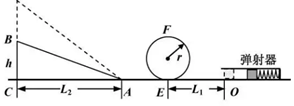
\includegraphics[]{img/image18.jpeg}
\end{center}

